\section{Introduction}\label{intro}\sloppy


Data cleaning is widely recognized as a major challenge in almost all forms of data analytics~\cite{nytimes}, and analysts may spend upwards of 80\% of the analysis effort to clean and prep the data.  A common form of data errors are those where attribute values are incorrect---these errors can vary from missing data, incorrect or biased values, misspellings, the concatenation of multiple attributes due to extraction errors, and more.  These errors must be fixed before being used by downstream applications such as SQL queries, visualizations, or machine learning models.    


Data cleaning is challenging because there is rarely a well-defined ground-truth. Instead, developers must both 1) characterize the data quality issues that affect their application, and 2) compose data cleaning programs to fix those issues.  However, this is challenging for two reasons.  First, developers often do not know the exact description nor the extend of the quality issues of their data up-front.  Instead, they examine analysis output and iteratively refine their understanding throughou the cleaning process~\cite{krishnan2016hilda}.  Second, developers must then translate these quality issues into concrete data cleaning programs that successfully fix the issues.  This is challenging because 

Second, developers must translate these quality characteristics into invocations of data cleaning operators to fix these errors.  However, even for a simple logical cleaning operator, such as outlier value imputation, there is a large space of physical cleaning options.  Which  outliers could utilize a fixed threshold, an unsupervised statistical model, a problem-specific model (e.g., of EEG signals~\cite{}), a based on constraints.  Each operation further burdens the developer with numerous choices to set its parameters---what threshold?  How many clusters? What model features?   Once the outliers have been detected, there is a similar buffet of options to actually replace the outlier value.     Unfortunately, data cleaning is challenging because even a single data set can have many different types of errors (e.g., outliers, constraint violations, duplicates, mis-spellings, incorrect orderings).




It is a human in the loop problem.


Specialized operators are tailored to specific error types and fix operators.

Pipelines are flexible, but requrie the developer to reason about a large search space.

Ideally, user primarily focuses on quantifying the error types, and the allows the system to generate cleaning programs, refining the search space as desired.

One promising approach is hyperparameter search.

It doesn't work.  Teaser example

Our paper 1) encodes cleaning objectives as a quality function, and provides tools for users to compose quality functions easily, 2) models cleaning as a sequential learning problem, 3) uses machine learning to dynamically prune the search space during the search process.  



Ultimately, data cleaning is a human-in-the-loop process driven by the user's domain expertise.  Thus, the input and output interfaces should be flexible and optimized for the user.   Users should be able to easily specify, and rapidly refine, potentially arbitrary {\it data-quality measures}.  It should also be easy to pick data transformation operators from a pre-existing library, or wrap specialized data cleaning libraries as user-defined operators.  To ensure that the system output is easy to understand, the system should generate simple programs composed of the user-specific transformation operators, rather than directly fixing the database contents.

A naive approach is to layer a black-box hyper-parameter tuning algorithm on an existing data cleaning framework.  The selection of operators, how they are combined, and how their parameters are set, can be modeled as a separate hyperparemeter that an optimization algorithm such as X, Y, or Z will explore.  The user's task is to specify and tune the optimization objective to lead the search towards an acceptable solution.   \ewu{THere's a gap here that I'm missing}

However this approach ignores important aspects of data cleaning problems that enable more efficient and flexible approaches.  First, data cleaning programs are often a sequence of transformations applied one after the other, thus the entire space of hyperparameters does not need to be learned jointly.  Second, a given transformation may be applied multiple times, whereas a black-box hyperparameter search algorithm would need to know up front the maximum set of trnsaforamiotns and the parameters. Third, the transformations are not commutative, and prior transformations can affect subsequent transformations.  This meoans that local decisions need to account for how they may affect later transformations.  


%Automated data cleaning takes as input a {\it specification} that characterizes the errors in the dataset, as well as a set of allowable {\it data transformations} (e.g., \texttt{set(rowi, attrj, val)}), and automatically applies these transformations to fix the errors.  

% Data  cleaning is composed of pipelines.  in some cases, the pipelines are largely fixed, and developers adjust the parameters of operators in the pipeline, or the pipeline itself, in response to changes in the input data.  In other cases, the core set of parameterized operators are know apriori, but the specific parameterization and pipeline of operators that should be run to achieve a desired data cleaning goal is not clear up front. The latter can happen at a regular basis as new data cleaning scenarios arise (say, due to new customers), a new data source is added to an analysis, or when a data source changes substantially.  In these cases, developers must construct the pipeline and parameterization in order to achieve an often ill-defined cleaning goal.





A starting point is the recent work on systems for \emph{hyperparameter tuning} for machine learning~\cite{li2017hyperband, sparks2017keystoneml, baylor2017tfx, golovin2017google, liaw2018tune}.
These systems are alternatively described as ``black box'' search algorithms as they make few assumptions about the underlying structure of the parameter space---simply put, generality at the cost of runtime.
In machine learning, the objective of the search process is clear: the prediction error on a validation set gives an estimate of accuracy. 
In data cleaning, there is a chicken-and-egg problem, where accuracy is defined in terms of recovering the true values of cells in a database, but knowing the true values in advance would defeat the purpose of cleaning.
In practice, we often use a proxy for accuracy such as the satisfaction of integrity constraints, how well it fits a statistical model, or accuracy on gold standard data.
Given one of these proxy accuracy metrics, is black-box hyperparameter tuning sufficient for applications in data cleaning optimization?

\begin{figure}[t]
\centering
 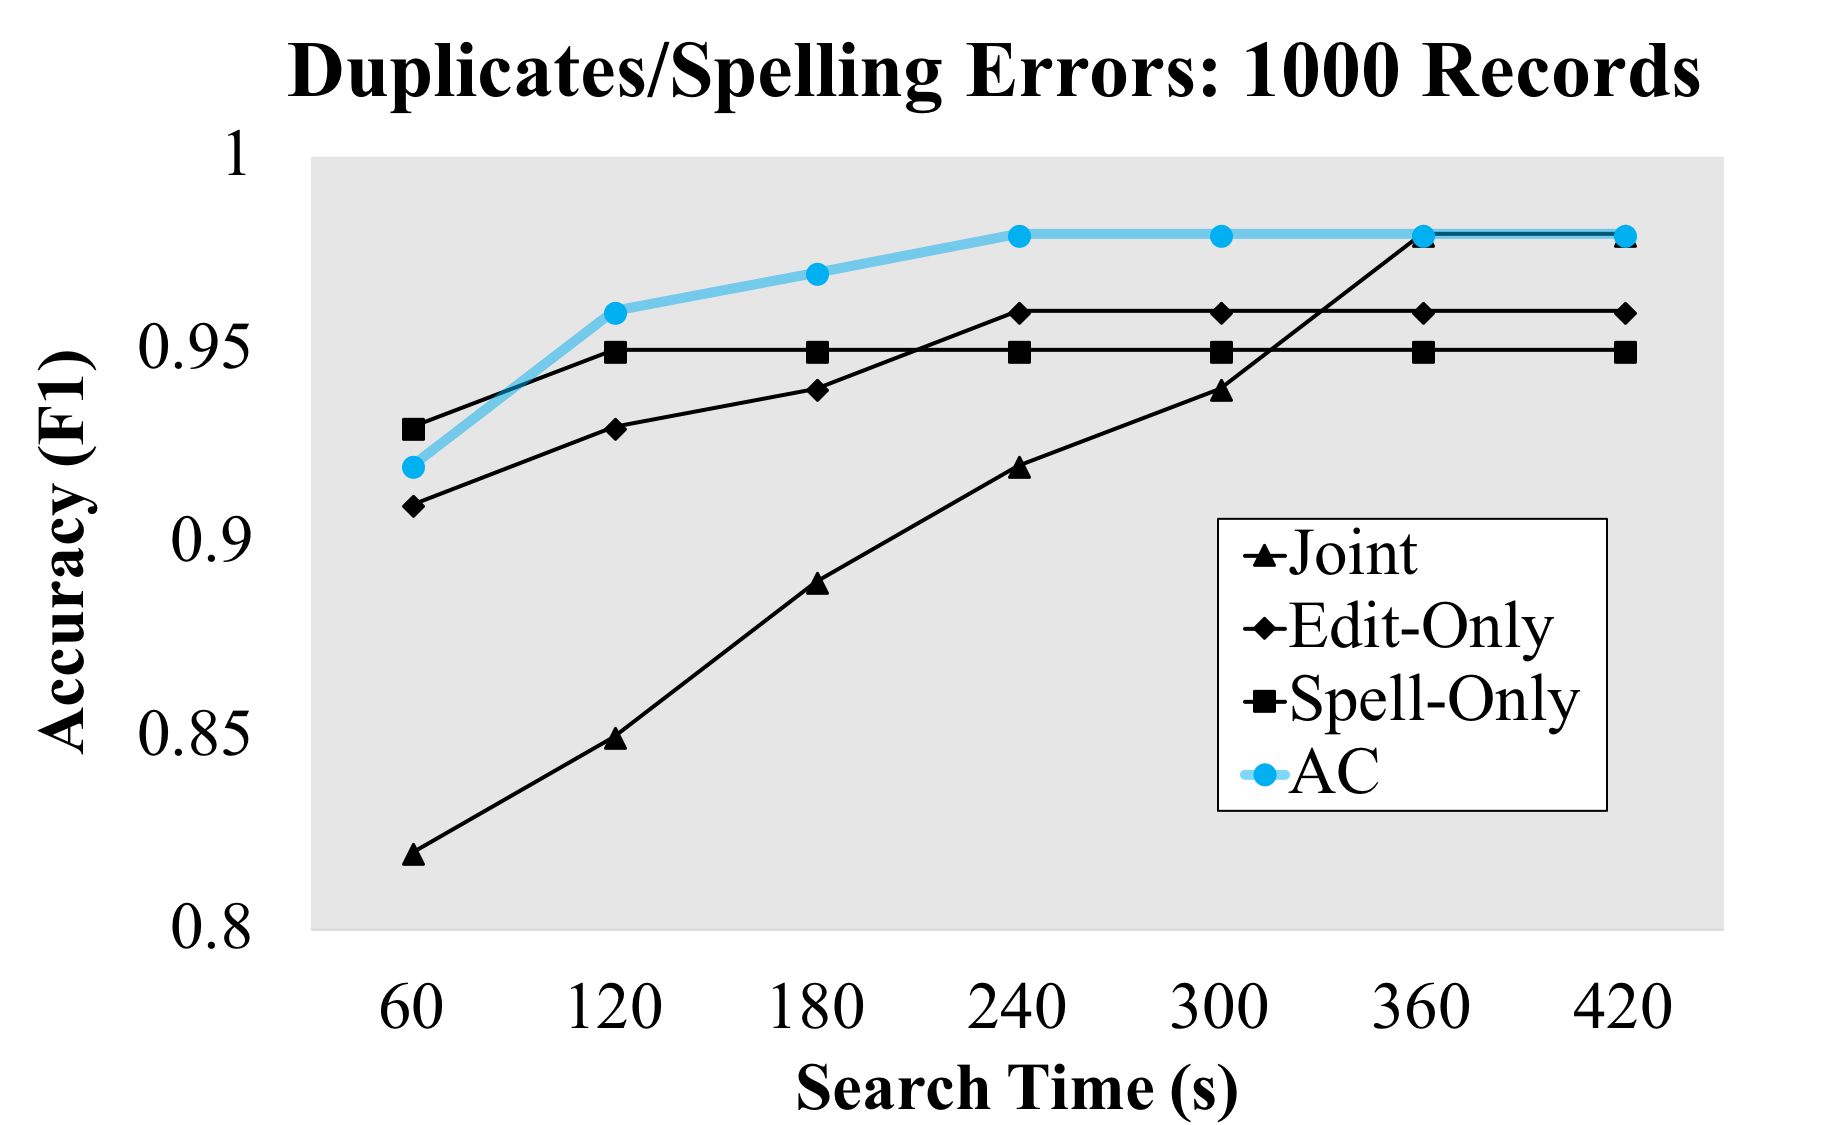
\includegraphics[width=0.9\columnwidth]{figures/teaser-experiment.png}
 \caption{\small 10\% of a dataset of dictionary words are duplicated with randomly generated spelling errors. The dataset is to be cleaned with a similarity matcher and a spell checker. Holistically, tuning the parameters of both with \textsf{python hyperopt} (Full) is inefficient due to interactions between the two data cleaning options. It takes over 3x the amount of search time for the joint optimization to exceed the best tuned single cleaning method (Edit and SpellCheck) \label{fig:teaser}}
\end{figure}

A subtle challenge is that existing black-box search algorithms would treat the entire data cleaning pipeline as a monolithic parametrized unit.
They do not explcitly reason about interactions between pipeline components, and those effects are latently captured in the parameter space and accuracy metric.
Consider a simple experiment: we have a dataset of 1000 dictionary words (10\% of which are duplicated with randomly generated spelling errors affecting 1-3 characters), and cleaned by an edit distance similarity matcher with a tunable threshold and a spell checker with a tunable recommendation parameter.
 One would expect that jointly optimizing over the entire pipeline (cascading the matcher and spellchecker) with a black-box optimizer is more reliable than simply tuning either of the single cleaning methods. 
Figure \ref{fig:teaser} (implemented with \textsf{python hyperopt}) illustrates that this is not exactly the case, it takes over 3x the amount of search time for the joint optimization to exceed the best tuned single cleaning method.
This experiment is designed such that there is redudancy in the pipeline, where duplicates can be resolved either by spellcheck or matching.
The joint optimization method wastes evaluation cycles exploring parameter settings where both techniques significantly overlap.


In this case, we are lucky; the joint optimization converges to a reasonable solution given enough time.
However, as we scale to more complex and larger scale problems, avoiding local optima becomes a daunting challenge.
Interactions between methods may not simply be redundancies, and improperly tuned techniques might even reverse the changes made by previous steps.
We arrived at a simple architecture to address this issue by rethinking the parameter search process.
For a given parameter setting, every data cleaning method in the pipeline suggests \emph{candidate} repairs to a dataset.
These repairs are aggregated into a large set of possible transformations to apply
Then, a meta-algorithm searches over sequential compositions of the set of generated candidates.
The size of the search space can be controlled by how many parameter settings are considered and how coarse- or fine-grained the repairs are.
This process allows the system to leverage partial repairs from the pipeline when beneficial and naturally avoid problems of redundancy.

More importantly, this generate-then-search process is specialized to the idiosyncrasies of data cleaning.
Data cleaning is fundamentally a form of constraint satisfaction---easy to verify but hard to satisfy.
So, candidate generation can be much more expensive than accuracy evaluation (e.g., for Denial Constraints).
Existing search algorithms implicitly pipeline these two steps; whereas, we decouple these two steps where candidate repairs can be generated in a separate thread and the search algorithm can proceed independently.


We implement this search framework in a system called \sys.
\sys is provided with a library of data cleaning components and specification of their free parameters. 
We assume that each component specifies its repairs in terms of cell-replacement, the same model as in recent systems like Holoclean~\cite{rekatsinas2017holoclean}.
A parameter generator thread supplies assignments to each of the data cleaning methods in the library and yields candidate repairs as they are generated to a set.
A greedy tree-search algorithm runs in parallel by sequencing candidate repairs and computing the resulting accuracy measure.
\sys can also execute in a divide-and-conquer fashion by generating candidate parameters on different partitions of data.
It also provides utilities for leveraging information across partitions, by learns a prediction model to estimate the expected improvement of different transformation operators (e.g., some library components might be irrelevant).  

\noindent Our contributions include:
\begin{itemize}[leftmargin=*, topsep=0mm, itemsep=0mm]
  \item Rethinking parameter optimization in data cleaning and data transformation with a novel candidate-search framework called \sys. \sys includes an API for specifying data cleaning operations as well as accuracy metrics.
  \item A suite of pragmatic optimizations, such as fast pruning using predictive models, multi-node parallelization, and data sharing to reduce network communication bottlenecks, that reduce the runtime by \ewu{XXX$\times$}.
  \item A systematic study of the benefits and limitations of \sys in terms of data cleaning accuracy (precision, recall), and the runtime.  We show that \sys can solve incremental refinements of the data quality measure $yyy\times$ faster than from scratch, and that \ewu{SOME OTHER FINDING}
\end{itemize}


